\documentclass{article}
\usepackage{graphicx} % Required for inserting images
\usepackage[top=0.9in, bottom=1in, left=1.5in, right=1.5in]{geometry}
\usepackage[utf8]{inputenc}
\usepackage[icelandic]{babel}
\usepackage[T1]{fontenc}
\usepackage[sc]{mathpazo}
\usepackage[parfill]{parskip}
\renewcommand{\baselinestretch}{1.2}
% Tables and lists
\usepackage{booktabs,tabularx}
\usepackage{multirow}
\usepackage{enumerate}
\usepackage{adjustbox}
\usepackage{multicol}
\usepackage{xcolor}
\usepackage{algpseudocode}
\usepackage{tikz}
\usepackage{nicefrac}
\usepackage{changepage}
\usetikzlibrary{arrows, positioning, calc, graphs}

% Math
\usepackage{amsmath, amsfonts, amssymb, amsthm}
% Graphics

\usepackage{graphicx}
\usepackage{tikz}
% Code environment
\usepackage{minted}
%\usepackage{bm}
%\usepackage{siunitx}
%\usepackage{animate}
%\usepackage{hyperref}
%\usepackage{movie15}
%\usepackage{multicol}
%\usepackage{changepage}
\title{Forritunarmál Einstaklingsverkefni 5}
\author{Ragnar Björn Ingvarsson, rbi3}
\tikzset{->, >=stealth', shorten >=1pt, node distance=2cm,thick, main node/.style={circle,draw,minimum size=3em}}

\begin{document}
\renewcommand\thepage{}
	
	\maketitle

	\newpage
	\setcounter{page}{1}
	\renewcommand\thepage{\arabic{page}}

	\section{}
	\begin{verbatim}
;; Notkun: (realpowrecursive x y)
;; Fyrir: x er tala, y er heiltala, y >= 0
;; Gildi: x^y
;;
;; Við nýtum okkur hér að ef y er slétt,
;; þá getum við skrifað (x^2)^{y/2} en ef
;; y er oddatala, þá getum við einnig skrifað
;; x(x^2)^{(y-1)/2}.
(define (realpowrecursive x y)
  (if (= y 0)
      1.0
      (if (= (remainder y 2) 0)
          (realpowrecursive (* x x) (/ y 2))
          (* x (realpowrecursive (* x x) (/ (- y 1) 2)))
          )
      )
  )
	\end{verbatim}
	\begin{center}
		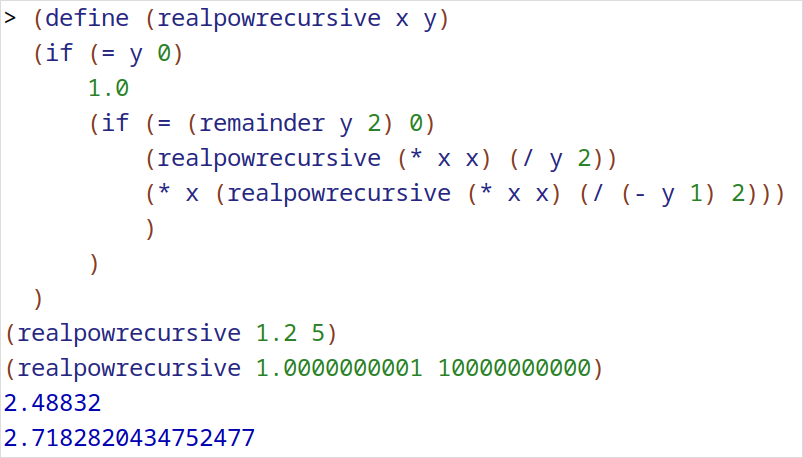
\includegraphics[scale=0.35]{realpow.png}
	\end{center}

	\newpage
	\section{}
	\begin{verbatim}
;; Notkun: (transpose-list z)
;; Fyrir: z er listi jafnlangra lista,
;; z=((x11 x12 ... x1N)
;; (x21 x22 ... x2N)
;; (x31 x32 ... x3N)
;; ...
;; (xM1 xM2 ... xMN)
;; )
;; Gildi: Listinn sem er byltingin
;; (transpose) af z, þ.e.
;; ((x11 x21 ... xM1)
;; (x12 x22 ... xM2)
;; (x13 x23 ... xM3)
;; ...
;; (x1N x2N ... xMN)
;; )
(define (transpose-list z)
  ;; Notkun: (head u)
  ;; Fyrir: u er listi (u1 u2 ... uN), N >= 0
  ;; Gildi: Ef N = 0 þá z[0][0], þ.e. x11,
  ;;        annars u1
  (define (head u)
    (if (null? (car u))
        (car (car z))
        (car u)
        )
    )
  ;; Notkun: (tail u)
  ;; Fyrir: u er listi (u1 u2 ... uN), N >= 0
  ;; Gildi: (u2 u3 ... uN)
  (define (tail u)
    (if (null? (car u))
        u
        (cdr u)
        )
    )
  (if (or (null? z) (null? (car z)))
      '()
      (cons (map head z) (transpose-list (map tail z)))
      )
  )
	\end{verbatim}
	\begin{center}
		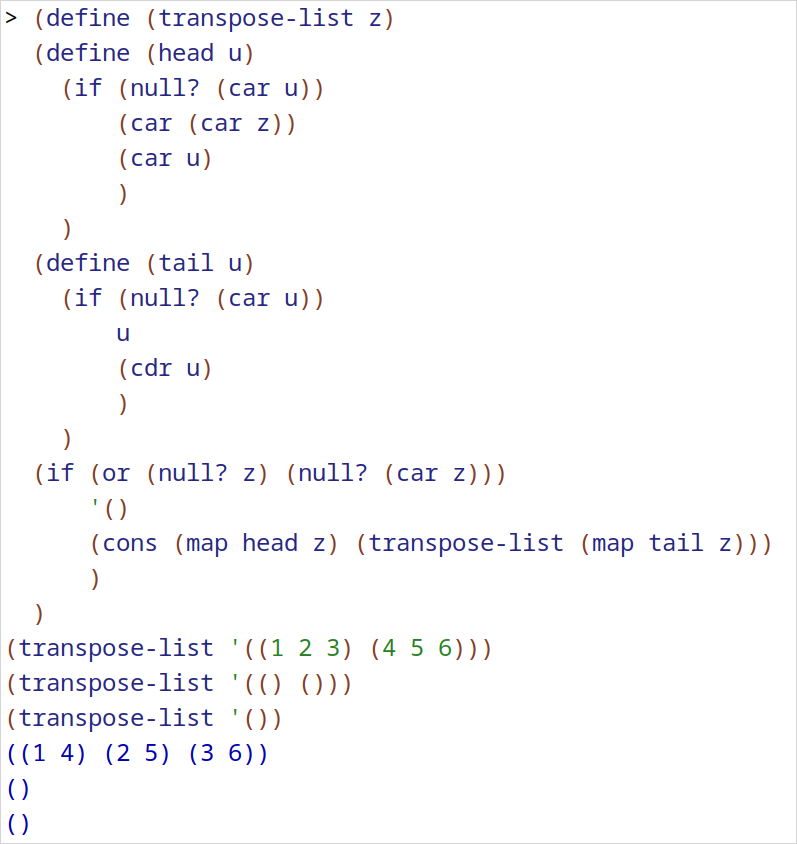
\includegraphics[scale=0.35]{transpose.png}
	\end{center}
\end{document}
